\documentclass{beamer}
\usetheme{Montpellier}
%
%Information to be included in the title page:
\title{Introdução à Séries Temporais}
\subtitle{Modelos Univariados Lineares}

\author{Macos Ferreira}
%
\institute{Universidade Mackenzie}
%
\date{2023}
%
%\logo{
\includegraphics[height=1cm]{mackenzie.png}}

%PACKAGES
\usepackage{enumerate}
\usepackage{graphicx}
\usepackage{multicol}
\graphicspath{ {./apresentacao_series_temporais/images/} }

%ADDITIONAL
\renewcommand{\figurename}{Fig.}
\setbeamertemplate{caption}[numbered]
\setbeamertemplate{bibliography item}{\insertbiblabel}


\begin{document}
	\frame{\titlepage}
	%
	\begin{frame}[allowframebreaks]
		\frametitle{Índice}
		\tableofcontents[hideallsubsections]
	\end{frame}
	%
	\section{1. Alguns Modelos de Séries Temporais}
	 \begin{frame}
		\frametitle{1.Lista dos Exemplos}
		\begin{itemize}
			\item<1-> Valores diários de índice de poluição em São Paulo \cite{morettin2018analise}
			\item<1-> Valores \textbf{mensais} de média de temperatura na cidade de Cananeia 
			\item<1-> Índice \textbf{diário} da Bovespa ([B]\textsuperscript{3})
			\item<1-> Precipitação pluviométrica Acumulada,\textbf{Anual} em Fortaleza(acumulado anual)
			\item<1-> Número médio \textbf{anual} de Manchas Solares(acumulado de manchas no ano)
			\item<1-> PIB Anual a preços de 1949			
		\end{itemize}		
	\end{frame}
	
	\subsection{1.2. Gráficos}
	% ---------------------------------------
	% graphics
	% ---------------------------------------
	
	% Poluicao
	\begin{frame}
		\frametitle{1.1. Índice de Poluição na Cidade de São Paulo}
		\begin{figure}[!ht]
			\centering
			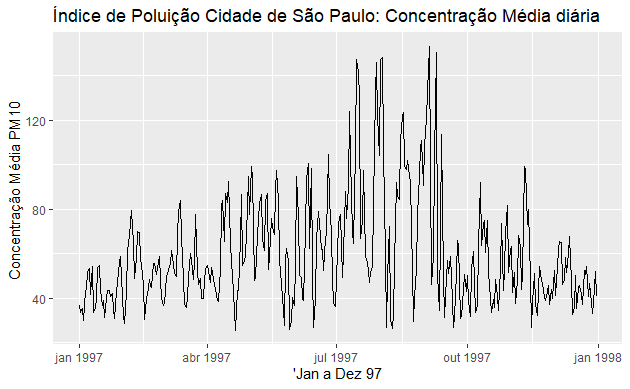
\includegraphics[width=0.7\linewidth]{apresentacao_series_temporais/images/Morettin_poluicao}
			\caption[Concentração de Poluentes-São Paulo:de 01/01/1997 à 31/12/1997]{Concentração de Poluentes-São Paulo:de 01/01/1997 à 31/12/1997}
			\label{fig:morettinpoluicao}
		\end{figure}	
	\end{frame}

	%Média de Temperatura Cananeia
	\begin{frame}
		\frametitle{1.2.Temperatura média na Cidade de Cananeia-SP}
		\begin{figure}[!ht]
			\centering
			\caption[Temperatura Média Cananeia:1977 a 1985]{Temperatura Média Cananeia:1977 a 1985}
			\label{fig:tempcananeia}
			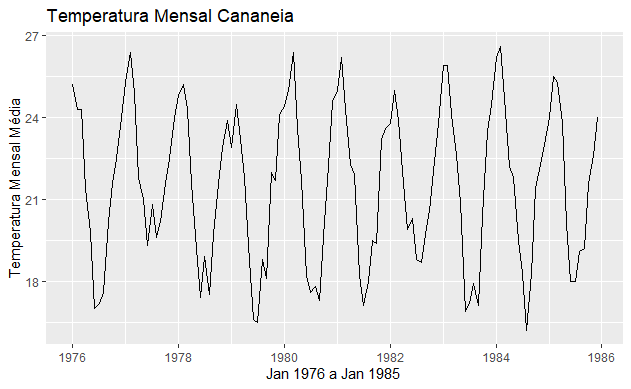
\includegraphics[width=0.7\linewidth]{apresentacao_series_temporais/images/temp_cananeia}
		\end{figure}
	\end{frame}
	
	% BOVESPA 
	\begin{frame}
		\frametitle{1.3. Índice Diário Bovespa}
		\begin{figure}[!ht]
				\centering
				\caption[Índice Diário Bovespa de 1998 à 2001]{Índice Diário Bovespa de 1998 à 2001}
				\label{fig:ibovespa}
				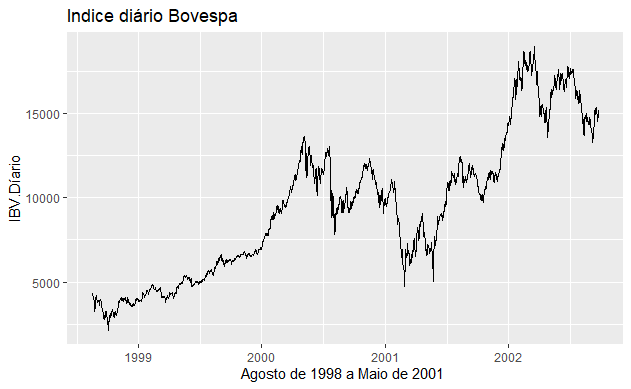
\includegraphics[width=0.7\linewidth]{apresentacao_series_temporais/images/IBOVESPA.D}
		\end{figure}
	\end{frame}

	% PRECIPITAÇÃO PLUVIOMÉTRICA ANUAL EM FORTALEZA
	\begin{frame}
		\frametitle{1.4. Precipitação Pluviométrica Anual em Fortaleza}
		\begin{figure}
			\centering
			\caption{Precipitação Pluviométrica média Anual Acumulada(mm) : Fortaleza (1849 a 1997)}
			\label{fig:fortaleza}
			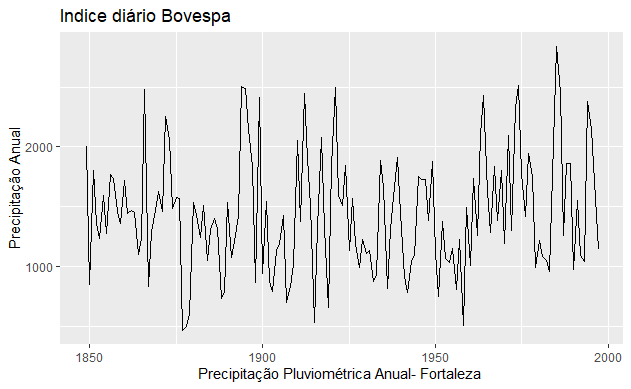
\includegraphics[width=0.7\linewidth]{apresentacao_series_temporais/images/Fortaleza}
		\end{figure}
	\end{frame}

	% NÚMERO MÉDIO ANUAL DE MANCHAS SOLARES
	\begin{frame}
		\begin{figure}
			\centering
			\caption{1.5. Número médio de Manchas Solares, desde 1749}
			\label{fig:manchas}
			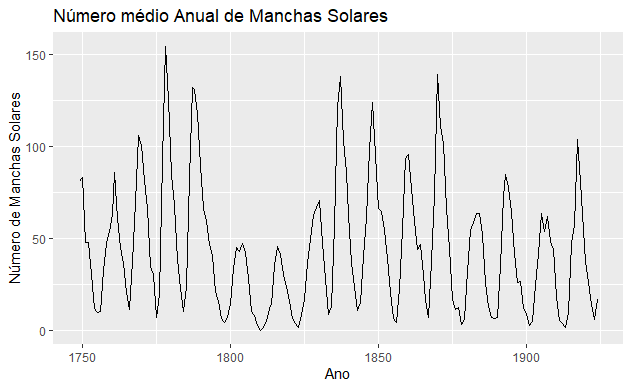
\includegraphics[width=0.7\linewidth]{apresentacao_series_temporais/images/manchas}
		\end{figure}
	\end{frame}

	%PIB ANUAL A PREÇOS DE 1949
	\begin{frame}
		\begin{figure}
			\centering
			\caption{1.5. PIB ANUAL Preços de 1949}
			\label{fig:pib}
			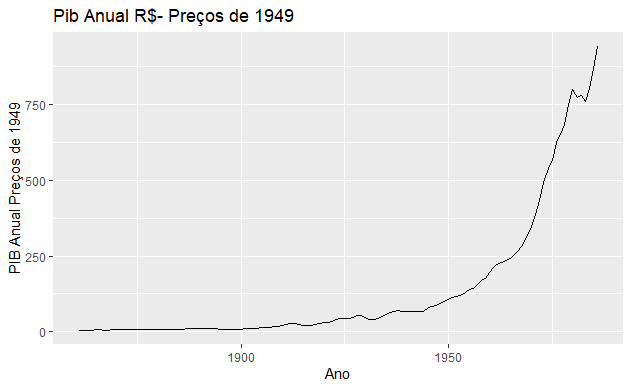
\includegraphics[width=0.7\linewidth]{apresentacao_series_temporais/images/pib}
		\end{figure}
	\end{frame}
	% sessão de enfoque para tratamentos de séries temporais
	\section{2.Enfoques de Tratamento de Séries Temporais}
	\begin{frame}
		\frametitle{2. Dois Enfoques para Abordagem de Séries Temporais}
		\begin{itemize}
			\item   Ver \cite{morettin2018analise,hamilton2020time,enders2008applied,shumway2000time}
		\end{itemize}
		\begin{columns}
			\begin{column}{0.5\textwidth}
				\begin{itemize}
					\item<1-> Domínio Temporal 
					\begin{itemize}
						\item<1-> Modelos Paramétricos
						\item<1-> Exemplo: Modelos ARIMA, na qual se estima os parâmetros dos valores do polinômio autoregressivo e de médias móveis, avaliando-se a significância de cada um deles				
					\end{itemize}
				\end{itemize}
			\end{column}
					   
		    \begin{column}{0.5\textwidth}
		    \begin{itemize}
		    	\item<1-> Domínio de Frequência( modelo não paramétrico)
		    	\begin{itemize}
		    		\item<1-> Consiste em decompor a série em componentes de frequência
		    		\item<1-> Exemplos:
		    		\begin{itemize}
		    			\item<1-> Análise Espectral
		    			\item<1->Aplicações em Física, Engenharia
		    		\end{itemize}	
		    	\end{itemize}
		    \end{itemize} 
		    \end{column}
	    
		\end{columns}	
	
	\end{frame}

	% Objetivos de Séries Temporais 
	\section{3. Objetivos da Modelagem de Séries Temporais}
	\begin{frame}
		\frametitle{3. Objetivos da Modelagem de Séries Temporais}
		\begin{itemize}
			\item<1-> Investigar o mecanismo Gerador da Série temporal
			\item<1-> Prever valores futuros da série, com base nos valores passados
			\item<1-> descrever o comportamento da série, usando-se, por exemplo, uma análise gráfica para averiguar tendências, ciclos, efeitos sazonais; analisar as correlações seriais, usando-se função de autocorrelação ou autocorrelação parcial(a ser visto adiante)
			\item<1-> Usar análise espectral de frequências para averiguar a periodicidade da série
		\end{itemize}
	\end{frame}

	% Transformação de Box-Cox
	\section{5. Transformações de Box-Cox}
	\begin{frame}
		\frametitle{5. Transformações de Box-Cox}
			\begin{itemize}
			\item<1-> Estabilizar a variância da série 
			\item<1-> Tornar o efeito sazonal aditivo 
			\begin{itemize}
				\item<1-> Tendências são comuns em séries financeiras e a variância pode aumentar, à medida que o tempo passa
			\end{itemize}
			
			\item<1-> A transformação matemática das variáveis, principalmente a transformação logarítmica ajuda a 'estabilizar' a variância e a 'normalizar' a série.
		\end{itemize}
		
	\end{frame}
	% SUBSECTION
	\subsection{As duas formas básicas de transformação}
	\begin{frame}
		\frametitle{As duas formas básicas de transformação}
		\begin{itemize}
			\item<1-> $	Z_{t}^{(\lambda)} = 
			\begin{cases}
				\frac{Z_{t}^{\lambda}-c}{\lambda}, se \lambda \neq 0,   \\
				
				\log{Z_{t}}, & \mbox{ se } \lambda = 0
			\end{cases}
			$		
		\end{itemize}
		%
		\begin{itemize} 
			\item<1-> $\lambda$ e c são parâmetros a serem estimados
		\end{itemize}
		%
		\begin{itemize} 
			\item<1->A transformação logarítmica é apropriada se o desvio padrão da série for proporcional à média , ( $\sigma \alpha \mu $)\cite{morettin2018analise}
		\end{itemize}
	\end{frame}
	% SUBSECTION
	\subsection{Escolhendo o valor de $\lambda$}
	\begin{frame}
		\frametitle{Escolhendo o valor de $\lambda$}
		\begin{itemize}
			\item<1-> \cite{morettin2018analise} sugere que para se ter ideia da transformação adequada, pode-se utilizar um gráfico, onde, no eixo das abcissas coloca-se o valor médio de um subconjunto de observações da série temporal e nas ordenadas, a amplitude de cada conjunto
			\item<1-> Seja $Z_{1},Z_{2},\dots,Z_{k}$ um subconjunto da série temporal, com $k$ observações
			\item<1-> Então: $ \bar{Z} = \frac{1}{k}\sum_{i=1}^{k} Z_{t_{i}} ; w= max(Z_{t_{i}}) - min(Z_{t_{i}})$
			\item<1-> O par $(\bar{Z},w)$ é um ponto no gráfico
		\end{itemize}
	\end{frame}

	\begin{frame}
		\frametitle{Escolhendo o valor de $\lambda$}
		\begin{itemize}
			\item<1-> Se $w$ for independente de $\bar{Z}$, os pontos estão espalhados ao redor de uma reta, paralela às abcissas e podemos aplicar $\lambda=1 \implies Z_{t}^{\lambda} = Z_{t} -1 $
			
			\item<1-> Se $w$ for diretamente proporcional à $\bar{Z}$ então podemos aplicar a transformação logarítmica, com $\lambda = 0 $
			
			\item<1-> Outros casos intermediários incluem $\lambda = -0.5 $ e $\lambda = 0.5 $
			\item<1-> para detalhes, ver \cite{box1964analysis}
		\end{itemize}
	\end{frame}
	% Ferramentas 
	\subsection{Alguns aplicativos para modelar séries temporais}
	\begin{frame}
		\frametitle{Ferramentas usadas em Séries Temporais}
		\begin{itemize}
			\item<1->  MINITAB
			\item<1->  SAS
			\item<1->  SPSS
			\item<1->  SPLUS
			\item<1->  Eviews
			\item<1->  Gretl
			\item<1->  R: Libraries astsa, forecast\cite{hyndman2018forecasting}, tpp, GeneCycle, moments,stats,fbProphet
			\item<1->  Python: fbProphet, Arima, AutoArima\cite{morettin2018analise}
			
		\end{itemize}
		
	\end{frame}

	\section{6.Modelos de Séries Temporais}
	\subsection{Processos Estocásticos}
	\frame{
		\frametitle{Processo Estocástico}
		\begin{itemize}
			\item<1-> Seja $\mathcal{T}$ um conjunto arbitrário 	 \cite{morettin2018analise}\cite{enders2008applied}
			\item<1-> $Z(t)$ uma variável aleatória
			\item<1-> Um processo estocástico é :
			\begin{itemize}
				\item<1-> Uma família de variáveis aleatórias
				\item<1-> $Z=\{\ Z(t), t \in \mathcal{T}  \}$
				\item<1-> As variáveis aleatórias estão definidas em um espaço de probabilidades $(\Omega,\mathcal{A},\mathcal{P})$
				\begin{itemize}
					\item<1-> $\Omega:$ espaço amostral
					\item<1-> $\mathcal{A}:$ Uma álgebra definida em $\Omega$
					\item<1-> $\mathcal{P}:$ Uma probabilidade, de modo que $\mathcal{P}(\Omega)=1$ 
				\end{itemize}
				\item<1-> $ \mathcal{T}$ definido em $\mathbb{Z}={\pm 1, \pm 2, \pm 3, ....}$ ou no conjunto dos reais $\mathbb{R}$
			\end{itemize}
		\end{itemize}
		
	}
	
	\subsection{Processos Estocásticos}
	% capítulo 2
	\frame{
		\frametitle{Exemplo de Um Processo Estocástico}
		\begin{itemize}
			\item<1-> \begin{figure}
				\centering
				\caption{Representação de uma realização um processo estocástico. No eixo $f_{Z}$ temos a probabilidade de $Z(t)$ ; no eixo t, os elementos de $t \in \mathcal{T}$; e, finalmente na ordenadas, o valor de $Z(t)$ de um membro particular da família de processos estocástico; a curva $\mu(t)$ descreve a trajetória das médias de $Z(t)$ para cada t; finalmente, cada $Z(t)$ pode ter uma distribuição de probabilidade diferente, embora o normal seja que a função de densidade de probabilidades seja a mesma\cite{morettin2018analise}.}
				\label{fig:familiadevariaveisaleatorias}
				\includegraphics[width=0.7\linewidth]{apresentacao_series_temporais/images/família_de_variaveis_aleatorias}
			\end{figure}
			
		\end{itemize}
		
	}
\subsection{Especificação do Processo Estocástico em termos formais}
\frame{
	\frametitle{Especificação formal de um processo estocástico}
	\begin{itemize}
		\item<1-> Sejam $ {Z}^{(1)}(t) ,{Z}^{(2)}(t) , \dots$ realizações específicas da família de processos estocásticos
		\item<1-> Sejam agora, $t_{1},t_{2},\dots,t_{n}$ elementos quaisquer de $\mathcal{T}$
		\item<1-> Seja ainda, $F(z_{1},z_{2},\dots,z_{n}) = \mathit{P}( Z(t_{1}) \leq z_{1},Z(t_{2}) \leq z_{2},\dots,Z(t_{n}) \leq z_{n}   ) $
		\item<1-> $\mathit{P}$ é a probabilidade que cada $t_{i}$ seja menor do que $z_{i}$
		\item<1-> Se conhecermos as distribuições de probabilidade das variáveis aleatórias $Z(t_{i})$ o processo estará especificado, desde que $\mathit{P}$ satisfaça as seguintes condições:
		\begin{itemize}
			\item<1-> Condição de simetria: para qualquer permutação $j_{1}, j_{2},\dots,j_{n}$ dos índices, então $F(z_{j_{1}},z_{j_{2}},\dots,z_{j_{n}}, t_{j_{1}},t_{j_{2}},\dots, t_{j_{n}})=F(z_{1},\dots,z_{n},t_{1},\dots,t_{n})$
		\end{itemize}
	\end{itemize}
}

\subsection{Especificação do Processo Estocástico em termos formais}
\frame{
	\frametitle{Especificação formal de um processo estocástico}
	\begin{itemize}
		\item<1-> Condição de Compatibilidade: se $m<n$ então $F(z_{1},z_{2},z_{m}; t_{1},t_{2},\dots,t_{m} )=F(z_{1},z_{2},z_{m},\infty;t_{1},t_{2},\dots,t_{m},t_{m+1},\dots)     $
		\item<1-> Na prática, é difícil conhecer a especificação completa de um processo estocástico, isto é, cada função de distribuição de probabilidade, e o que se faz é estudar os momentos geradores do processo, em particular, os de baixa ordem
		\begin{itemize}
			\item<1-> Valor médio $\mu_{t}$
			\item<1-> Variância $ \sigma_{t} $
			\item<1-> Covariância :$COV(X_{t},X_{s})=\gamma(t,s)$
		\end{itemize}
		
	\end{itemize}
}

\subsection{Especificação do Processo Estocástico em termos formais}
\frame{
	\begin{itemize}
		\item<1->\begin{figure}
			\centering
			\caption{Representação de vários elementos de uma família de um processo estocástico Z, com realizações $Z^{(1)},Z^{(2)}, Z^{(3)},Z^{(4)}$}
			\label{fig:familiasvariaveisaleatorias2}
			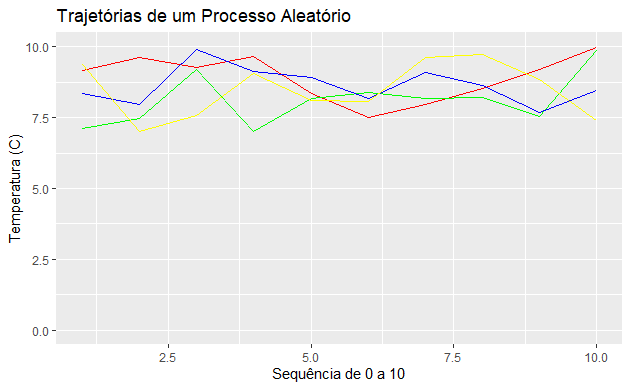
\includegraphics[width=0.7\linewidth]{apresentacao_series_temporais/images/familias_variaveis_aleatorias_2}
		\end{figure}
		
	\end{itemize}
}


\subsection{Processos Estacionários}
\frame{
	\frametitle{Processos Estacionários}
	\framesubtitle{Processos Estritamente Estacionários}
	\begin{itemize}
		\item<1-> Processos Estritamente Estacionários
		\begin{itemize}
			\item<1-> Um processo estocástico $Z =\{Z(t),t \in \mathcal{T}\}$ é dito estritamente estacionário se suas estatísticas não são afetadas pela escolha da origem dos tempos ou devido à translação do tempo.
			\item<1-> Dito mais formalmente, todas as suas distribuições finito-dimensionais permanecem as mesmas sob translação no tempo, i.e:
			\begin{itemize}
				\item<1-> $\mathit{F}(z_{1},z_{2},\dots,z_{n}; t_{1}+ \tau, t_{2}+ \tau,\dots,t_{n}+ \tau,  )=\mathit{F}(z_{1},z_{2},\dots,z_{n}; t_{1}, t_{2},\dots,t_{n}  )$ 
			\end{itemize}
			\item<1-> As distribuições são invariantes sob uma translação. No caso de uma distribuição unidimensional com momentos finitos, então, a média e variância são constantes finitas, isto é:
			\item<1-> $\mu(t) = \mu ; V(t)=\sigma^{2}$
			\item<1-> As distribuições bidimensionais dependem de $t_{2} - t_{1}$ de modo que $\gamma(t_{1},t_{2})=\gamma(|t_{1}-t_{2}|)$
		\end{itemize}	
	\end{itemize}
}
\subsection{Processos Estacionários}
\frame{
	\frametitle{Processos Estacionários}
	\framesubtitle{Processos Processos Fracamente Estacionários}
	\begin{itemize}
		\item<1-> Processos Fracamente Estacionários
		\begin{itemize}
			\item<1-> Um processo $Z=\{Z(t), t \in \mathcal{T}\}$ é dito fracamente estacionário ou estacionário de segunda ordem se e somente se:
			\item<1-> $E\{Z(t)\}= \mu(t)= \mu$; constante para todo $t\in \mathcal{T}$
			\item<1-> $E\{Z^{2}(t)\}\}< \infty $ para todo $t\in \mathcal{T}$
			\item<1-> $ \gamma(t_{1},t_{2}) =Cov(Z(t_{1},t_{2}))  $ é função de $|t_{1} - t_{2}|$
		\end{itemize}
		\item<1-> Em um processo fracamente estacionário, somente se requer condições sobre os momentos de primeira e segunda ordem e não sobre a função de distribuição finito-dimensional. \cite{fischer1982series} 
		\item<1-> As distribuições finito-dimensionais podem não ser as mesmas, mas se as médias, variâncias forem as mesmas e a covariância só depender da diferença dos tempos, então a série é fracamente estacionária
	\end{itemize}
}
\section{7.Função de Autocovariância}
\subsection{Autocovariância}
\frame{
	\frametitle{Função de Autocovariância}
	\begin{itemize}
		\item<1-> Define-se a função de autocovariâcia(facv) com defasagem $k$ da série como :
		\item<1-> $\gamma_{k}=Cov(Z_{t},Z_{t+k}) = E[(Z_{t}-\mu_{t})(Z_{t+k}- \mu_{t+k})]$
		\item<-1> Se a série é estacionária, então $\mu_{t}=\mu_{t+k}=\mu$
		\item<1-> Se a série for estacionária, então as seguintes propriedades são válidas para a função de autocovariância:
		\item<-1> $\gamma_{0}>0$
		\item<-1> $\gamma_{t}=\gamma_{-t}$
		\item<-1> $|\gamma_{t}|\leq \gamma_{0}$
		\item<-1> $\sum\limits_{j=1}^{n}\sum\limits_{k=1}^{n}{a_{j}.a_{k}.\gamma_{\tau_{j} -\tau_{k} }  } \geq 0, \forall a_{k}, a_{j}  \in \mathbb{R}$
		\item<-1> essa última propriedade define que $\gamma_{\tau}$ é não negativa definida
	\end{itemize}
	
}

%%%%%%%%%%%%%%%%%%%%%%
% exemplos de processos estocásticos
%%%%%%%%%%%%%%%%%%%%%%
\subsection{Exemplos de Processos Estocásticos}
\begin{frame}[allowframebreaks]
	\frametitle{Exemplos de Processos Estocásticos}
	\begin{itemize}
		\item<1->Sequência Aleatória
		\begin{itemize}
			\item<1-> Seja $X=\{ X_{n};n=1,2,3,\dots,\}$  uma sequência de variáveis aleatórias, definidas todas em um espaço amostral $\Omega$;
			\item<1-> Sendo assim,  $\mathcal{T}=\{1,2,\dots\}$
			\item<1-> Para $n \geq 1$:
			\begin{itemize}
				\item<1-> $\mathit{P}(X_{1}=a_{1},\dots,X_{n}=a_{n})=\mathit{P}(X_{1}=a_{1})\times\mathit{P}(X_{2}=a_{2}|X_{1}=a_{1},)\times \dots \times \mathit{P}(X_{n}=a_{n}| X_{1}=a_{1},X_{2}=a_{2},\dots,X_{n-1}=a_{n-1} )$ 
			\end{itemize} 
		\begin{itemize}
			\item<1-> Os $a_{j}$ representam estados do processo
			\item<1-> Se a sequência $X(t)$ for de variáveis aleatórias, mutuamente independentes, então
			$\mathit{P}(X_{1}=a_{1},\dots,X_{n}=a_{n}) = \prod_{i=1}^{n}\mathit{P}(X_{i}=a_{i})$ 
		\end{itemize}
		\item<1-> Além disso, se todas as variáveis aleatórias $X_{i}$ tiverem a mesma distribuição, então a sequência de v.a é dita independente e igualmente distribuída
		\end{itemize}
	\item<1-> O processo $X$ é estacionário, nesse caso : $\mathit{E}(X_{i})=\mu;  Var(X_{i})=\sigma^{2}; \gamma_{\tau}=Cov\{X_{n},X_{n+\tau}\}$ se $\tau \neq 0$
	\item<1-> Se $\gamma_{s}=Cov\{\varepsilon_{t},\varepsilon_{s}\}=0$, então o processo $\{\varepsilon_{t},t \in \mathbb{Z} \}$ é dito um ruído branco.
	\item<1-> Então, um processo estocástico aleatório é tal que as variáveis aleatórias são i.i.d(independente e identicamente distribuídas) e não correlacionadas entre si
	\item<1-> Sua facv ( função de autocovariância ) é tal que somente $Var(\varepsilon_{t}) = \sigma^{2}$
	\begin{figure}
		\centering
		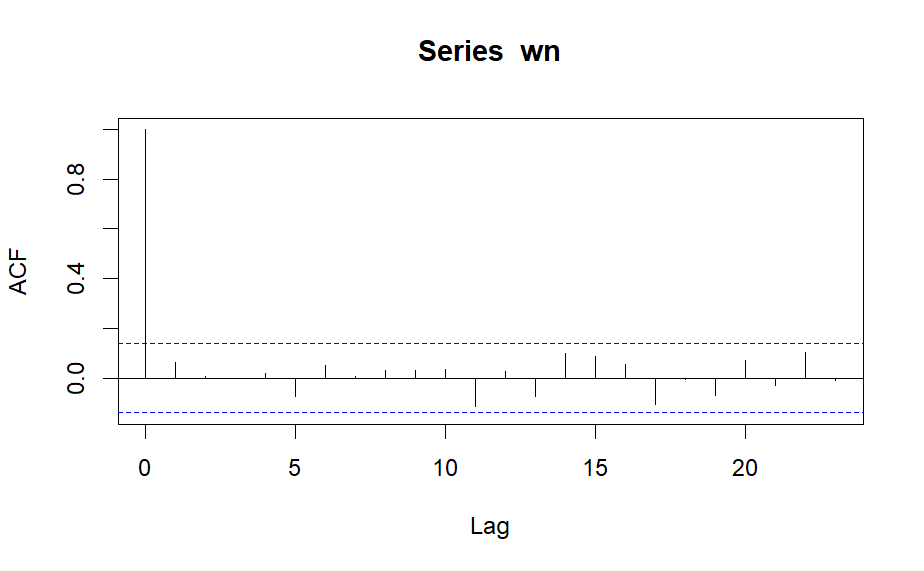
\includegraphics[width=0.5\linewidth]{apresentacao_series_temporais/images/acf_wn}
		\caption[Função de Auto Covariância de um ruído branco]{Note que todos os outros valores da fac são iguais a zero, exceto o valor de $Cov(\epsilon_{t},\epsilon_{t})=\sigma^{2}$}
		\label{fig:acfwn}
	\end{figure}
	
	 
	\end{itemize}
\end{frame}

\begin{frame}[allowframebreaks]
	\frametitle{Exemplos de Processos Estocásticos II: passeio aleatório}
	\begin{itemize}
		\item<1->Seja $\varepsilon_{t}, t \geq 1$ uma sequência aleatória cujas variáveis são i.i.d , com média $\mu$ e variância $\sigma_{\varepsilon}^2$ 
		\item<1-> Defina a sequência \[X_{t} = \sum_{i=1}^{t}\varepsilon_{i}\] 
		\item<1-> Então, \[ E(X_{t}) = t\mu_{t} \] e \[ Var(X_{t}) = t \sigma_{\varepsilon}^{2}\]
		\item<1-> Além disso, \[ \gamma_{X}(t_{1},t_{2}) = \sigma_{\varepsilon} min(t_{1},t_{2})\]
		\item<1-> Esse processo denomina-se passeio aleatório ou causal
		\item<1-> Esse processo não é estacionário
	\end{itemize}
    \begin{figure}
    	\centering
    	\caption{Um passeio aleatório.}
    	\label{fig:random}
    	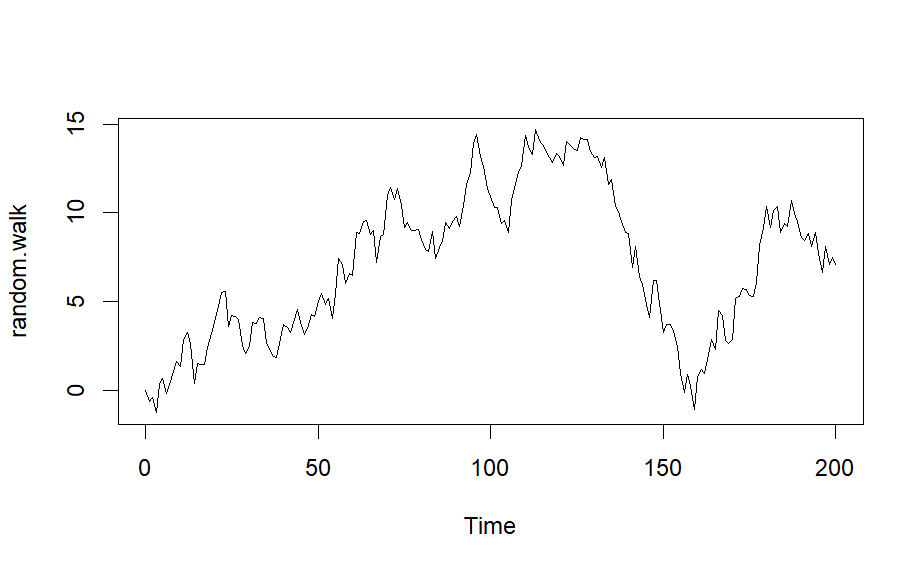
\includegraphics[width=0.7\linewidth]{apresentacao_series_temporais/images/random.walk}
    \end{figure}
    
\end{frame}

%%%%%%%%%%%%%%%%%%%%%%%%%%%%%%%%%%%%%%%%%%%%%%
% MODELO ARIMA
%%%%%%%%%%%%%%%%%%%%%%%%%%%%%%%%%%%%%%%%%%%%%%

\section{8.Modelos Arima}
\subsection{Metodologia de Box-Jenkins}
\begin{frame}
	\frametitle{'Metodologia de Box-Jenkins'} 
	\begin{itemize}
		\item<1->\begin{figure}
			\centering
			\caption{Metodologia Box-Jenkins}
			\label{fig:boxjenkinsmethodology}
			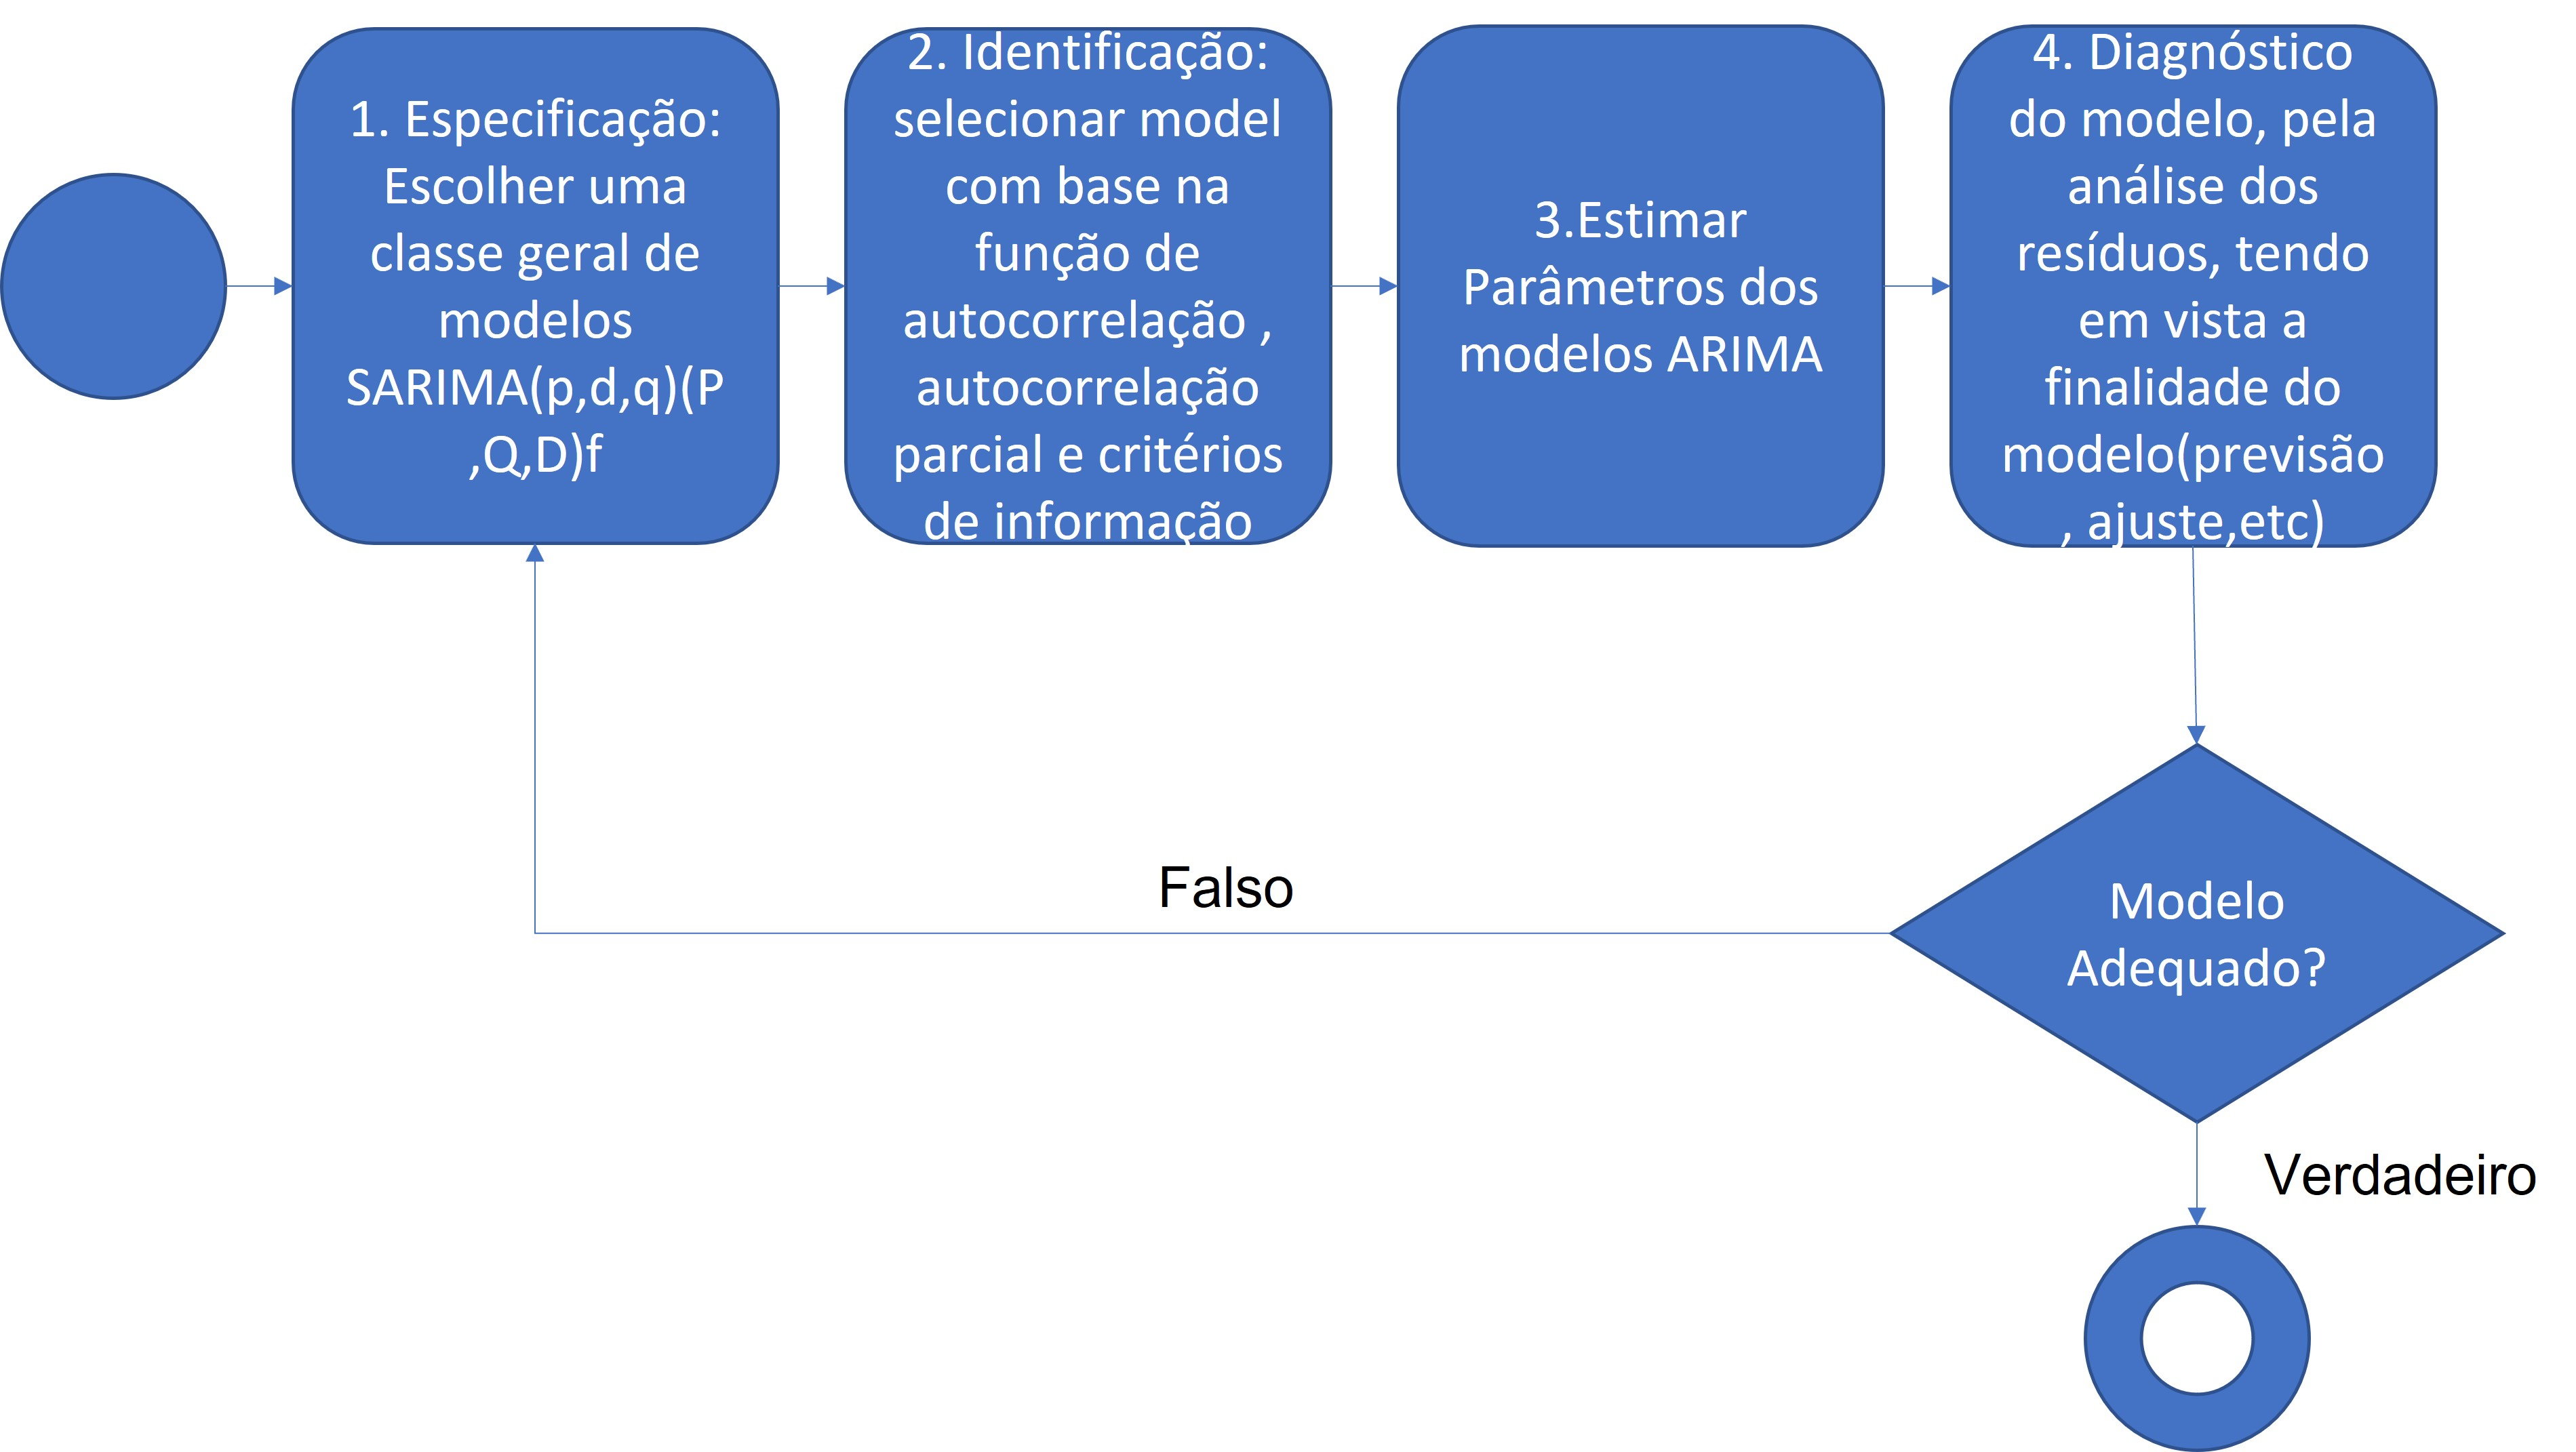
\includegraphics[width=0.7\linewidth]{apresentacao_series_temporais/images/box_jenkins_methodology}
		\end{figure}
		
	\end{itemize}
\end{frame}
\subsection{Metodologia de Box-Jenkins}
\begin{frame}
	\begin{itemize}
		\item<1-> Proposto por Box \& Jenkins em 1976 
		\item<1-> Consiste em ajustar modelos autoregressivos integrados e de médias móveis
		\item<1-> Pode ser estendido a modelos sazonais $SARIMA(p,d,q)(P,D,Q)_{f}$
		
	\end{itemize}
\end{frame}
\subsection{Operadores}
\begin{frame}
	\begin{itemize}
		\item<1-> Operador Translação para Trás(behind)
		\begin{itemize}
			\item $BZ_{t} = Z_{t-1}; B^{m}Z_{t} = Z-{t-m}  $
		\end{itemize}
		\item<1-> Operador Translação para Frente(future)
			\begin{itemize}
				\item $FZ_{t}=Z_{t+1}; F^{m}Z_{t}=Z_{t+m}$
			\end{itemize}
		\item<1-> Operador Diferença
			\begin{itemize}
				\item $ \Delta Z_{t}=Z_{t} - Z_{t-1} = (1-B)Z_{t}$ 
			\end{itemize}
		\item<1-> Operador Soma
			\begin{itemize}
				\item 	$SZ_{t} =  \sum_{J=0}^{\infty} Z_{t-j} = Z_{t} + Z_{t-1}+\dots+ = (1+B+B^{2}+\dots)Z_{t} $
				\item Se $\|B\|<1 \implies SZ_{t} = (1-B)^{-1}Z_{t}=\Delta^{-1}Z_{t}$
			\end{itemize}
		
	\end{itemize}
\end{frame}
    
    %%%%%%%%%%%%%%%%%%%%%%%%%%%%%%%%%%%%%%%%%%%%%%%%%%%%%%%
	% Sessões Finais: Referência bibliográfica
	%%%%%%%%%%%%%%%%%%%%%%%%%%%%%%%%%%%%%%%%%%%%%%%%%%%%%%%
	\section{Bibliografia}
	\begin{frame}[allowframebreaks]
		\frametitle{Bibliografia}
		\bibliography{./bibliografia}
		\bibliographystyle{ieeetr}
	\end{frame}
\end{document}
